\documentclass[1p]{elsarticle_modified}
%\bibliographystyle{elsarticle-num}

%\usepackage[colorlinks]{hyperref}
%\usepackage{abbrmath_seonhwa} %\Abb, \Ascr, \Acal ,\Abf, \Afrak
\usepackage{amsfonts}
\usepackage{amssymb}
\usepackage{amsmath}
\usepackage{amsthm}
\usepackage{scalefnt}
\usepackage{amsbsy}
\usepackage{kotex}
\usepackage{caption}
\usepackage{subfig}
\usepackage{color}
\usepackage{graphicx}
\usepackage{xcolor} %% white, black, red, green, blue, cyan, magenta, yellow
\usepackage{float}
\usepackage{setspace}
\usepackage{hyperref}

\usepackage{tikz}
\usetikzlibrary{arrows}

\usepackage{multirow}
\usepackage{array} % fixed length table
\usepackage{hhline}

%%%%%%%%%%%%%%%%%%%%%
\makeatletter
\renewcommand*\env@matrix[1][\arraystretch]{%
	\edef\arraystretch{#1}%
	\hskip -\arraycolsep
	\let\@ifnextchar\new@ifnextchar
	\array{*\c@MaxMatrixCols c}}
\makeatother %https://tex.stackexchange.com/questions/14071/how-can-i-increase-the-line-spacing-in-a-matrix
%%%%%%%%%%%%%%%

\usepackage[normalem]{ulem}

\newcommand{\msout}[1]{\ifmmode\text{\sout{\ensuremath{#1}}}\else\sout{#1}\fi}
%SOURCE: \msout is \stkout macro in https://tex.stackexchange.com/questions/20609/strikeout-in-math-mode

\newcommand{\cancel}[1]{
	\ifmmode
	{\color{red}\msout{#1}}
	\else
	{\color{red}\sout{#1}}
	\fi
}

\newcommand{\add}[1]{
	{\color{blue}\uwave{#1}}
}

\newcommand{\replace}[2]{
	\ifmmode
	{\color{red}\msout{#1}}{\color{blue}\uwave{#2}}
	\else
	{\color{red}\sout{#1}}{\color{blue}\uwave{#2}}
	\fi
}

\newcommand{\Sol}{\mathcal{S}} %segment
\newcommand{\D}{D} %diagram
\newcommand{\A}{\mathcal{A}} %arc


%%%%%%%%%%%%%%%%%%%%%%%%%%%%%5 test

\def\sl{\operatorname{\textup{SL}}(2,\Cbb)}
\def\psl{\operatorname{\textup{PSL}}(2,\Cbb)}
\def\quan{\mkern 1mu \triangleright \mkern 1mu}

\theoremstyle{definition}
\newtheorem{thm}{Theorem}[section]
\newtheorem{prop}[thm]{Proposition}
\newtheorem{lem}[thm]{Lemma}
\newtheorem{ques}[thm]{Question}
\newtheorem{cor}[thm]{Corollary}
\newtheorem{defn}[thm]{Definition}
\newtheorem{exam}[thm]{Example}
\newtheorem{rmk}[thm]{Remark}
\newtheorem{alg}[thm]{Algorithm}

\newcommand{\I}{\sqrt{-1}}
\begin{document}

%\begin{frontmatter}
%
%\title{Boundary parabolic representations of knots up to 8 crossings}
%
%%% Group authors per affiliation:
%\author{Yunhi Cho} 
%\address{Department of Mathematics, University of Seoul, Seoul, Korea}
%\ead{yhcho@uos.ac.kr}
%
%
%\author{Seonhwa Kim} %\fnref{s_kim}}
%\address{Center for Geometry and Physics, Institute for Basic Science, Pohang, 37673, Korea}
%\ead{ryeona17@ibs.re.kr}
%
%\author{Hyuk Kim}
%\address{Department of Mathematical Sciences, Seoul National University, Seoul 08826, Korea}
%\ead{hyukkim@snu.ac.kr}
%
%\author{Seokbeom Yoon}
%\address{Department of Mathematical Sciences, Seoul National University, Seoul, 08826,  Korea}
%\ead{sbyoon15@snu.ac.kr}
%
%\begin{abstract}
%We find all boundary parabolic representation of knots up to 8 crossings.
%
%\end{abstract}
%\begin{keyword}
%    \MSC[2010] 57M25 
%\end{keyword}
%
%\end{frontmatter}

%\linenumbers
%\tableofcontents
%
\newcommand\colored[1]{\textcolor{white}{\rule[-0.35ex]{0.8em}{1.4ex}}\kern-0.8em\color{red} #1}%
%\newcommand\colored[1]{\textcolor{white}{ #1}\kern-2.17ex	\textcolor{white}{ #1}\kern-1.81ex	\textcolor{white}{ #1}\kern-2.15ex\color{red}#1	}

{\Large $\underline{12n_{0596}~(K12n_{0596})}$}

\setlength{\tabcolsep}{10pt}
\renewcommand{\arraystretch}{1.6}
\vspace{1cm}\begin{tabular}{m{100pt}>{\centering\arraybackslash}m{274pt}}
\multirow{5}{120pt}{
	\centering
	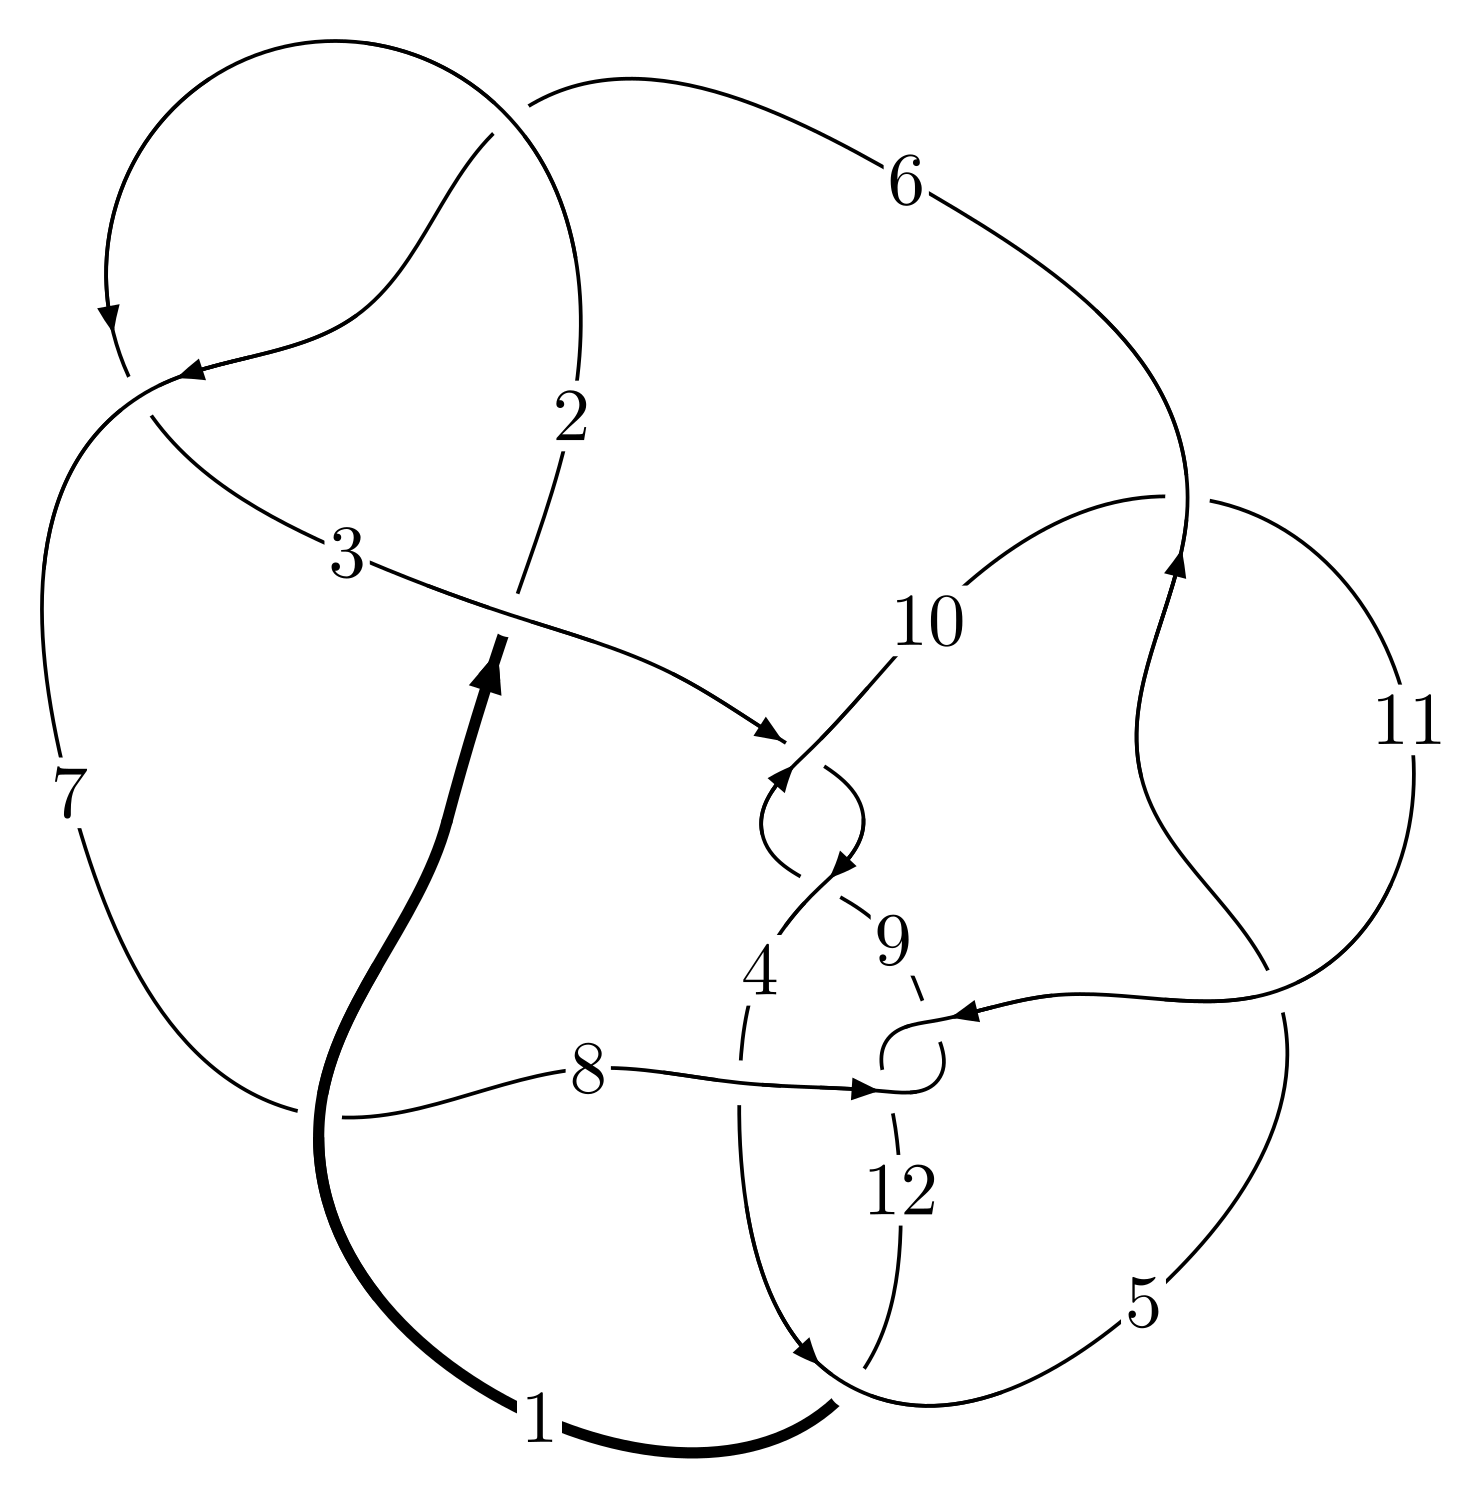
\includegraphics[width=112pt]{../../../GIT/diagram.site/Diagrams/png/2685_12n_0596.png}\\
\ \ \ A knot diagram\footnotemark}&
\allowdisplaybreaks
\textbf{Linearized knot diagam} \\
\cline{2-2}
 &
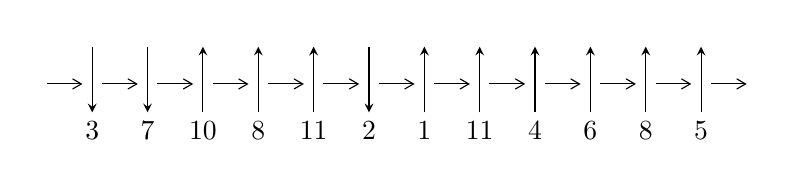
\begin{tikzpicture}[x=20pt, y=17pt]
	% nodes
	\node (C0) at (0, 0) {};
	\node (C1) at (1, 0) {};
	\node (C1U) at (1, +1) {};
	\node (C1D) at (1, -1) {3};

	\node (C2) at (2, 0) {};
	\node (C2U) at (2, +1) {};
	\node (C2D) at (2, -1) {7};

	\node (C3) at (3, 0) {};
	\node (C3U) at (3, +1) {};
	\node (C3D) at (3, -1) {10};

	\node (C4) at (4, 0) {};
	\node (C4U) at (4, +1) {};
	\node (C4D) at (4, -1) {8};

	\node (C5) at (5, 0) {};
	\node (C5U) at (5, +1) {};
	\node (C5D) at (5, -1) {11};

	\node (C6) at (6, 0) {};
	\node (C6U) at (6, +1) {};
	\node (C6D) at (6, -1) {2};

	\node (C7) at (7, 0) {};
	\node (C7U) at (7, +1) {};
	\node (C7D) at (7, -1) {1};

	\node (C8) at (8, 0) {};
	\node (C8U) at (8, +1) {};
	\node (C8D) at (8, -1) {11};

	\node (C9) at (9, 0) {};
	\node (C9U) at (9, +1) {};
	\node (C9D) at (9, -1) {4};

	\node (C10) at (10, 0) {};
	\node (C10U) at (10, +1) {};
	\node (C10D) at (10, -1) {6};

	\node (C11) at (11, 0) {};
	\node (C11U) at (11, +1) {};
	\node (C11D) at (11, -1) {8};

	\node (C12) at (12, 0) {};
	\node (C12U) at (12, +1) {};
	\node (C12D) at (12, -1) {5};
	\node (C13) at (13, 0) {};

	% arrows
	\draw[->,>={angle 60}]
	(C0) edge (C1) (C1) edge (C2) (C2) edge (C3) (C3) edge (C4) (C4) edge (C5) (C5) edge (C6) (C6) edge (C7) (C7) edge (C8) (C8) edge (C9) (C9) edge (C10) (C10) edge (C11) (C11) edge (C12) (C12) edge (C13) ;	\draw[->,>=stealth]
	(C1U) edge (C1D) (C2U) edge (C2D) (C3D) edge (C3U) (C4D) edge (C4U) (C5D) edge (C5U) (C6U) edge (C6D) (C7D) edge (C7U) (C8D) edge (C8U) (C9D) edge (C9U) (C10D) edge (C10U) (C11D) edge (C11U) (C12D) edge (C12U) ;
	\end{tikzpicture} \\
\hhline{~~} \\& 
\textbf{Solving Sequence} \\ \cline{2-2} 
 &
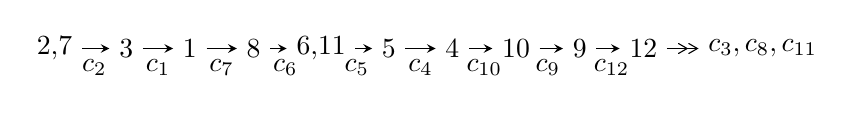
\begin{tikzpicture}[x=23pt, y=7pt]
	% node
	\node (A0) at (-1/8, 0) {2,7};
	\node (A1) at (1, 0) {3};
	\node (A2) at (2, 0) {1};
	\node (A3) at (3, 0) {8};
	\node (A4) at (65/16, 0) {6,11};
	\node (A5) at (41/8, 0) {5};
	\node (A6) at (49/8, 0) {4};
	\node (A7) at (57/8, 0) {10};
	\node (A8) at (65/8, 0) {9};
	\node (A9) at (73/8, 0) {12};
	\node (C1) at (1/2, -1) {$c_{2}$};
	\node (C2) at (3/2, -1) {$c_{1}$};
	\node (C3) at (5/2, -1) {$c_{7}$};
	\node (C4) at (7/2, -1) {$c_{6}$};
	\node (C5) at (37/8, -1) {$c_{5}$};
	\node (C6) at (45/8, -1) {$c_{4}$};
	\node (C7) at (53/8, -1) {$c_{10}$};
	\node (C8) at (61/8, -1) {$c_{9}$};
	\node (C9) at (69/8, -1) {$c_{12}$};
	\node (A10) at (11, 0) {$c_{3},c_{8},c_{11}$};

	% edge
	\draw[->,>=stealth]	
	(A0) edge (A1) (A1) edge (A2) (A2) edge (A3) (A3) edge (A4) (A4) edge (A5) (A5) edge (A6) (A6) edge (A7) (A7) edge (A8) (A8) edge (A9) ;
	\draw[->>,>={angle 60}]	
	(A9) edge (A10);
\end{tikzpicture} \\ 

\end{tabular} \\

\footnotetext{
The image of knot diagram is generated by the software ``\textbf{Draw programme}" developed by Andrew Bartholomew(\url{http://www.layer8.co.uk/maths/draw/index.htm\#Running-draw}), where we modified some parts for our purpose(\url{https://github.com/CATsTAILs/LinksPainter}).
}\phantom \\ \newline 
\centering \textbf{Ideals for irreducible components\footnotemark of $X_{\text{par}}$} 
 
\begin{align*}
I^u_{1}&=\langle 
5 u^{27}+23 u^{26}+\cdots+2 b+26,\;11 u^{27}+49 u^{26}+\cdots+4 a+44,\;u^{28}+5 u^{27}+\cdots+26 u+4\rangle \\
I^u_{2}&=\langle 
76637 u^8 a^3+229871 u^8 a^2+\cdots-157797 a-344895,\;-2 u^8 a^3-2 u^8 a^2+\cdots+a+9,\\
\phantom{I^u_{2}}&\phantom{= \langle  }u^9- u^8-2 u^7+3 u^6+u^5-3 u^4+2 u^3- u+1\rangle \\
I^u_{3}&=\langle 
- u^{16}-2 u^{15}+\cdots+b-3,\;-2 u^{16}-2 u^{15}+\cdots+a-3,\\
\phantom{I^u_{3}}&\phantom{= \langle  }u^{17}-5 u^{15}+12 u^{13}-15 u^{11}+9 u^9+u^7-4 u^5- u^4+2 u^3+2 u^2-1\rangle \\
\\
\end{align*}
\raggedright * 3 irreducible components of $\dim_{\mathbb{C}}=0$, with total 81 representations.\\
\footnotetext{All coefficients of polynomials are rational numbers. But the coefficients are sometimes approximated in decimal forms when there is not enough margin.}
\newpage
\renewcommand{\arraystretch}{1}
\centering \section*{I. $I^u_{1}= \langle 5 u^{27}+23 u^{26}+\cdots+2 b+26,\;11 u^{27}+49 u^{26}+\cdots+4 a+44,\;u^{28}+5 u^{27}+\cdots+26 u+4 \rangle$}
\flushleft \textbf{(i) Arc colorings}\\
\begin{tabular}{m{7pt} m{180pt} m{7pt} m{180pt} }
\flushright $a_{2}=$&$\begin{pmatrix}1\\0\end{pmatrix}$ \\
\flushright $a_{7}=$&$\begin{pmatrix}0\\u\end{pmatrix}$ \\
\flushright $a_{3}=$&$\begin{pmatrix}1\\u^2\end{pmatrix}$ \\
\flushright $a_{1}=$&$\begin{pmatrix}- u^2+1\\- u^4\end{pmatrix}$ \\
\flushright $a_{8}=$&$\begin{pmatrix}u^5-2 u^3+u\\u^7- u^5+u\end{pmatrix}$ \\
\flushright $a_{6}=$&$\begin{pmatrix}u\\u\end{pmatrix}$ \\
\flushright $a_{11}=$&$\begin{pmatrix}-\frac{11}{4} u^{27}-\frac{49}{4} u^{26}+\cdots-\frac{283}{4} u-11\\-\frac{5}{2} u^{27}-\frac{23}{2} u^{26}+\cdots-\frac{145}{2} u-13\end{pmatrix}$ \\
\flushright $a_{5}=$&$\begin{pmatrix}u^{27}+\frac{7}{2} u^{26}+\cdots+\frac{23}{2} u+\frac{5}{2}\\\frac{7}{2} u^{27}+\frac{31}{2} u^{26}+\cdots+\frac{163}{2} u+14\end{pmatrix}$ \\
\flushright $a_{4}=$&$\begin{pmatrix}-3 u^{27}-\frac{19}{2} u^{26}+\cdots-\frac{15}{2} u+\frac{1}{2}\\-\frac{11}{2} u^{27}-\frac{43}{2} u^{26}+\cdots-\frac{155}{2} u-12\end{pmatrix}$ \\
\flushright $a_{10}=$&$\begin{pmatrix}-\frac{15}{4} u^{27}-\frac{61}{4} u^{26}+\cdots-\frac{331}{4} u-13\\-\frac{7}{2} u^{27}-\frac{29}{2} u^{26}+\cdots-\frac{169}{2} u-15\end{pmatrix}$ \\
\flushright $a_{9}=$&$\begin{pmatrix}-3 u^{27}-\frac{23}{2} u^{26}+\cdots-\frac{121}{2} u-\frac{19}{2}\\-\frac{5}{2} u^{27}-\frac{19}{2} u^{26}+\cdots-\frac{113}{2} u-10\end{pmatrix}$ \\
\flushright $a_{12}=$&$\begin{pmatrix}\frac{5}{4} u^{27}+\frac{15}{4} u^{26}+\cdots+\frac{61}{4} u+3\\-\frac{1}{2} u^{27}-\frac{5}{2} u^{26}+\cdots+\frac{3}{2} u+1\end{pmatrix}$\\&\end{tabular}
\flushleft \textbf{(ii) Obstruction class $= -1$}\\~\\
\flushleft \textbf{(iii) Cusp Shapes $= u^{27}+7 u^{26}+11 u^{25}-24 u^{24}-95 u^{23}-48 u^{22}+228 u^{21}+408 u^{20}-13 u^{19}-797 u^{18}-888 u^{17}+232 u^{16}+1501 u^{15}+1333 u^{14}-346 u^{13}-1800 u^{12}-1511 u^{11}+137 u^{10}+1416 u^9+1255 u^8+153 u^7-670 u^6-686 u^5-222 u^4+135 u^3+209 u^2+110 u+38$}\\~\\
\newpage\renewcommand{\arraystretch}{1}
\flushleft \textbf{(iv) u-Polynomials at the component}\newline \\
\begin{tabular}{m{50pt}|m{274pt}}
Crossings & \hspace{64pt}u-Polynomials at each crossing \\
\hline $$\begin{aligned}c_{1}\end{aligned}$$&$\begin{aligned}
&u^{28}+15 u^{27}+\cdots+44 u+16
\end{aligned}$\\
\hline $$\begin{aligned}c_{2},c_{6}\end{aligned}$$&$\begin{aligned}
&u^{28}-5 u^{27}+\cdots-26 u+4
\end{aligned}$\\
\hline $$\begin{aligned}c_{3},c_{5},c_{9}\\c_{10}\end{aligned}$$&$\begin{aligned}
&u^{28}+9 u^{26}+\cdots- u+1
\end{aligned}$\\
\hline $$\begin{aligned}c_{4},c_{12}\end{aligned}$$&$\begin{aligned}
&u^{28}- u^{27}+\cdots-2 u+1
\end{aligned}$\\
\hline $$\begin{aligned}c_{7}\end{aligned}$$&$\begin{aligned}
&u^{28}-15 u^{27}+\cdots-2082 u+196
\end{aligned}$\\
\hline $$\begin{aligned}c_{8},c_{11}\end{aligned}$$&$\begin{aligned}
&u^{28}+24 u^{27}+\cdots+4608 u+512
\end{aligned}$\\
\hline
\end{tabular}\\~\\
\newpage\renewcommand{\arraystretch}{1}
\flushleft \textbf{(v) Riley Polynomials at the component}\newline \\
\begin{tabular}{m{50pt}|m{274pt}}
Crossings & \hspace{64pt}Riley Polynomials at each crossing \\
\hline $$\begin{aligned}c_{1}\end{aligned}$$&$\begin{aligned}
&y^{28}-3 y^{27}+\cdots+3856 y+256
\end{aligned}$\\
\hline $$\begin{aligned}c_{2},c_{6}\end{aligned}$$&$\begin{aligned}
&y^{28}-15 y^{27}+\cdots-44 y+16
\end{aligned}$\\
\hline $$\begin{aligned}c_{3},c_{5},c_{9}\\c_{10}\end{aligned}$$&$\begin{aligned}
&y^{28}+18 y^{27}+\cdots+13 y+1
\end{aligned}$\\
\hline $$\begin{aligned}c_{4},c_{12}\end{aligned}$$&$\begin{aligned}
&y^{28}-39 y^{27}+\cdots-42 y+1
\end{aligned}$\\
\hline $$\begin{aligned}c_{7}\end{aligned}$$&$\begin{aligned}
&y^{28}+21 y^{27}+\cdots+8244 y+38416
\end{aligned}$\\
\hline $$\begin{aligned}c_{8},c_{11}\end{aligned}$$&$\begin{aligned}
&y^{28}-14 y^{27}+\cdots-2883584 y+262144
\end{aligned}$\\
\hline
\end{tabular}\\~\\
\newpage\flushleft \textbf{(vi) Complex Volumes and Cusp Shapes}
$$\begin{array}{c|c|c}  
\text{Solutions to }I^u_{1}& \I (\text{vol} + \sqrt{-1}CS) & \text{Cusp shape}\\
 \hline 
\begin{aligned}
u &= \phantom{-}0.929249 + 0.341636 I \\
a &= \phantom{-}0.193428 - 0.245481 I \\
b &= -0.030096 - 0.588079 I\end{aligned}
 & -1.44836 - 1.32384 I & \phantom{-}0.695067 + 0.255787 I \\ \hline\begin{aligned}
u &= \phantom{-}0.929249 - 0.341636 I \\
a &= \phantom{-}0.193428 + 0.245481 I \\
b &= -0.030096 + 0.588079 I\end{aligned}
 & -1.44836 + 1.32384 I & \phantom{-}0.695067 - 0.255787 I \\ \hline\begin{aligned}
u &= -0.660663 + 0.703535 I \\
a &= -0.684282 + 0.401431 I \\
b &= \phantom{-}0.508694 + 0.182176 I\end{aligned}
 & \phantom{-}5.08436 - 3.47708 I & \phantom{-}7.23263 + 2.58361 I \\ \hline\begin{aligned}
u &= -0.660663 - 0.703535 I \\
a &= -0.684282 - 0.401431 I \\
b &= \phantom{-}0.508694 - 0.182176 I\end{aligned}
 & \phantom{-}5.08436 + 3.47708 I & \phantom{-}7.23263 - 2.58361 I \\ \hline\begin{aligned}
u &= -0.978713 + 0.436112 I \\
a &= -0.573780 + 0.856820 I \\
b &= -0.23105 + 1.41378 I\end{aligned}
 & -0.59221 + 3.85896 I & \phantom{-}5.41585 - 8.89544 I \\ \hline\begin{aligned}
u &= -0.978713 - 0.436112 I \\
a &= -0.573780 - 0.856820 I \\
b &= -0.23105 - 1.41378 I\end{aligned}
 & -0.59221 - 3.85896 I & \phantom{-}5.41585 + 8.89544 I \\ \hline\begin{aligned}
u &= -0.893353 + 0.642807 I \\
a &= \phantom{-}0.439255 - 0.143317 I \\
b &= \phantom{-}0.481145 - 1.329810 I\end{aligned}
 & \phantom{-}4.40206 + 8.59519 I & \phantom{-}6.36570 - 7.75404 I \\ \hline\begin{aligned}
u &= -0.893353 - 0.642807 I \\
a &= \phantom{-}0.439255 + 0.143317 I \\
b &= \phantom{-}0.481145 + 1.329810 I\end{aligned}
 & \phantom{-}4.40206 - 8.59519 I & \phantom{-}6.36570 + 7.75404 I \\ \hline\begin{aligned}
u &= -0.181084 + 0.864099 I \\
a &= \phantom{-}2.35580 + 0.19920 I \\
b &= \phantom{-}0.657053 - 0.345268 I\end{aligned}
 & \phantom{-}0.30413 - 10.11890 I & \phantom{-}5.46914 + 5.28623 I \\ \hline\begin{aligned}
u &= -0.181084 - 0.864099 I \\
a &= \phantom{-}2.35580 - 0.19920 I \\
b &= \phantom{-}0.657053 + 0.345268 I\end{aligned}
 & \phantom{-}0.30413 + 10.11890 I & \phantom{-}5.46914 - 5.28623 I\\
 \hline 
 \end{array}$$\newpage$$\begin{array}{c|c|c}  
\text{Solutions to }I^u_{1}& \I (\text{vol} + \sqrt{-1}CS) & \text{Cusp shape}\\
 \hline 
\begin{aligned}
u &= -0.390931 + 0.790393 I \\
a &= \phantom{-}0.553034 - 0.988547 I \\
b &= -0.088477 - 0.180368 I\end{aligned}
 & \phantom{-}3.66685 + 0.77577 I & \phantom{-}5.01952 - 3.31127 I \\ \hline\begin{aligned}
u &= -0.390931 - 0.790393 I \\
a &= \phantom{-}0.553034 + 0.988547 I \\
b &= -0.088477 + 0.180368 I\end{aligned}
 & \phantom{-}3.66685 - 0.77577 I & \phantom{-}5.01952 + 3.31127 I \\ \hline\begin{aligned}
u &= -0.046181 + 0.865065 I \\
a &= -1.71050 - 0.23913 I \\
b &= -0.600654 + 0.312900 I\end{aligned}
 & -5.04513 - 2.20112 I & \phantom{-}6.66836 + 3.09691 I \\ \hline\begin{aligned}
u &= -0.046181 - 0.865065 I \\
a &= -1.71050 + 0.23913 I \\
b &= -0.600654 - 0.312900 I\end{aligned}
 & -5.04513 + 2.20112 I & \phantom{-}6.66836 - 3.09691 I \\ \hline\begin{aligned}
u &= \phantom{-}1.194960 + 0.139644 I \\
a &= \phantom{-}0.479609 - 0.801194 I \\
b &= \phantom{-}0.64008 - 1.70137 I\end{aligned}
 & -1.55027 - 3.30862 I & \phantom{-}0.08727 + 3.64392 I \\ \hline\begin{aligned}
u &= \phantom{-}1.194960 - 0.139644 I \\
a &= \phantom{-}0.479609 + 0.801194 I \\
b &= \phantom{-}0.64008 + 1.70137 I\end{aligned}
 & -1.55027 + 3.30862 I & \phantom{-}0.08727 - 3.64392 I \\ \hline\begin{aligned}
u &= -1.104270 + 0.595120 I \\
a &= -0.695565 + 0.302010 I \\
b &= -1.190600 + 0.700335 I\end{aligned}
 & \phantom{-}1.56113 + 4.41097 I & \phantom{-}1.00210 - 1.17558 I \\ \hline\begin{aligned}
u &= -1.104270 - 0.595120 I \\
a &= -0.695565 - 0.302010 I \\
b &= -1.190600 - 0.700335 I\end{aligned}
 & \phantom{-}1.56113 - 4.41097 I & \phantom{-}1.00210 + 1.17558 I \\ \hline\begin{aligned}
u &= \phantom{-}1.251710 + 0.341500 I \\
a &= \phantom{-}0.02594 - 1.65411 I \\
b &= -0.77011 - 2.56071 I\end{aligned}
 & -4.19391 + 6.08731 I & \phantom{-}0.85731 - 2.80136 I \\ \hline\begin{aligned}
u &= \phantom{-}1.251710 - 0.341500 I \\
a &= \phantom{-}0.02594 + 1.65411 I \\
b &= -0.77011 + 2.56071 I\end{aligned}
 & -4.19391 - 6.08731 I & \phantom{-}0.85731 + 2.80136 I\\
 \hline 
 \end{array}$$\newpage$$\begin{array}{c|c|c}  
\text{Solutions to }I^u_{1}& \I (\text{vol} + \sqrt{-1}CS) & \text{Cusp shape}\\
 \hline 
\begin{aligned}
u &= -1.206160 + 0.542493 I \\
a &= -0.15086 + 2.22381 I \\
b &= -0.02581 + 3.45703 I\end{aligned}
 & -2.7661 + 15.2558 I & \phantom{-}2.52297 - 8.38664 I \\ \hline\begin{aligned}
u &= -1.206160 - 0.542493 I \\
a &= -0.15086 - 2.22381 I \\
b &= -0.02581 - 3.45703 I\end{aligned}
 & -2.7661 - 15.2558 I & \phantom{-}2.52297 + 8.38664 I \\ \hline\begin{aligned}
u &= \phantom{-}1.251980 + 0.436921 I \\
a &= -0.149674 + 1.280100 I \\
b &= \phantom{-}0.44752 + 1.88854 I\end{aligned}
 & -8.98786 - 2.38473 I & \phantom{-}3.28316 + 0.77142 I \\ \hline\begin{aligned}
u &= \phantom{-}1.251980 - 0.436921 I \\
a &= -0.149674 - 1.280100 I \\
b &= \phantom{-}0.44752 - 1.88854 I\end{aligned}
 & -8.98786 + 2.38473 I & \phantom{-}3.28316 - 0.77142 I \\ \hline\begin{aligned}
u &= -1.237260 + 0.486713 I \\
a &= \phantom{-}0.03375 - 1.83518 I \\
b &= -0.13153 - 2.67194 I\end{aligned}
 & -8.62321 + 7.05383 I & \phantom{-}4.15719 - 6.57682 I \\ \hline\begin{aligned}
u &= -1.237260 - 0.486713 I \\
a &= \phantom{-}0.03375 + 1.83518 I \\
b &= -0.13153 + 2.67194 I\end{aligned}
 & -8.62321 - 7.05383 I & \phantom{-}4.15719 + 6.57682 I \\ \hline\begin{aligned}
u &= -0.429297 + 0.384695 I \\
a &= \phantom{-}1.133840 + 0.097257 I \\
b &= \phantom{-}0.333840 - 0.315853 I\end{aligned}
 & \phantom{-}0.916737 - 0.202146 I & \phantom{-}11.22373 + 1.78332 I \\ \hline\begin{aligned}
u &= -0.429297 - 0.384695 I \\
a &= \phantom{-}1.133840 - 0.097257 I \\
b &= \phantom{-}0.333840 + 0.315853 I\end{aligned}
 & \phantom{-}0.916737 + 0.202146 I & \phantom{-}11.22373 - 1.78332 I\\
 \hline 
 \end{array}$$\newpage\newpage\renewcommand{\arraystretch}{1}
\centering \section*{II. $I^u_{2}= \langle 7.66\times10^{4} a^{3} u^{8}+2.30\times10^{5} a^{2} u^{8}+\cdots-1.58\times10^{5} a-3.45\times10^{5},\;-2 u^8 a^3-2 u^8 a^2+\cdots+a+9,\;u^9- u^8-2 u^7+3 u^6+u^5-3 u^4+2 u^3- u+1 \rangle$}
\flushleft \textbf{(i) Arc colorings}\\
\begin{tabular}{m{7pt} m{180pt} m{7pt} m{180pt} }
\flushright $a_{2}=$&$\begin{pmatrix}1\\0\end{pmatrix}$ \\
\flushright $a_{7}=$&$\begin{pmatrix}0\\u\end{pmatrix}$ \\
\flushright $a_{3}=$&$\begin{pmatrix}1\\u^2\end{pmatrix}$ \\
\flushright $a_{1}=$&$\begin{pmatrix}- u^2+1\\- u^4\end{pmatrix}$ \\
\flushright $a_{8}=$&$\begin{pmatrix}u^5-2 u^3+u\\u^7- u^5+u\end{pmatrix}$ \\
\flushright $a_{6}=$&$\begin{pmatrix}u\\u\end{pmatrix}$ \\
\flushright $a_{11}=$&$\begin{pmatrix}a\\-0.348260 a^{3} u^{8}-1.04460 a^{2} u^{8}+\cdots+0.717073 a+1.56730\end{pmatrix}$ \\
\flushright $a_{5}=$&$\begin{pmatrix}0.0201175 a^{3} u^{8}-0.189537 a^{2} u^{8}+\cdots+0.953476 a+0.606425\\1.18312 a^{3} u^{8}+0.607006 a^{2} u^{8}+\cdots-0.223129 a-0.845472\end{pmatrix}$ \\
\flushright $a_{4}=$&$\begin{pmatrix}0.102078 a^{3} u^{8}+0.780534 a^{2} u^{8}+\cdots+0.252298 a+2.71609\\1.10786 a^{3} u^{8}+0.872901 a^{2} u^{8}+\cdots+0.474304 a+0.368532\end{pmatrix}$ \\
\flushright $a_{10}=$&$\begin{pmatrix}0.574324 a^{3} u^{8}+0.498198 a^{2} u^{8}+\cdots+1.36008 a-1.45711\\0.226064 a^{3} u^{8}-0.546399 a^{2} u^{8}+\cdots+1.07715 a+0.110190\end{pmatrix}$ \\
\flushright $a_{9}=$&$\begin{pmatrix}-0.946496 a^{3} u^{8}-0.481503 a^{2} u^{8}+\cdots+1.29709 a+0.301795\\-1.23084 a^{3} u^{8}-0.992111 a^{2} u^{8}+\cdots-0.666073 a+0.450292\end{pmatrix}$ \\
\flushright $a_{12}=$&$\begin{pmatrix}0.704404 a^{3} u^{8}+0.679020 a^{2} u^{8}+\cdots+1.31993 a-0.641679\\-0.0950072 a^{3} u^{8}-0.862513 a^{2} u^{8}+\cdots+1.36519 a+2.02857\end{pmatrix}$\\&\end{tabular}
\flushleft \textbf{(ii) Obstruction class $= -1$}\\~\\
\flushleft \textbf{(iii) Cusp Shapes $= 4 u^7-8 u^5+4 u^4+8 u^3-4 u^2+4 u+6$}\\~\\
\newpage\renewcommand{\arraystretch}{1}
\flushleft \textbf{(iv) u-Polynomials at the component}\newline \\
\begin{tabular}{m{50pt}|m{274pt}}
Crossings & \hspace{64pt}u-Polynomials at each crossing \\
\hline $$\begin{aligned}c_{1}\end{aligned}$$&$\begin{aligned}
&(u^9+5 u^8+12 u^7+15 u^6+9 u^5- u^4-4 u^3-2 u^2+u+1)^4
\end{aligned}$\\
\hline $$\begin{aligned}c_{2},c_{6}\end{aligned}$$&$\begin{aligned}
&(u^9+u^8-2 u^7-3 u^6+u^5+3 u^4+2 u^3- u-1)^4
\end{aligned}$\\
\hline $$\begin{aligned}c_{3},c_{5},c_{9}\\c_{10}\end{aligned}$$&$\begin{aligned}
&u^{36}+u^{35}+\cdots-1540 u-431
\end{aligned}$\\
\hline $$\begin{aligned}c_{4},c_{12}\end{aligned}$$&$\begin{aligned}
&u^{36}- u^{35}+\cdots-2656 u-751
\end{aligned}$\\
\hline $$\begin{aligned}c_{7}\end{aligned}$$&$\begin{aligned}
&(u^9+3 u^8+8 u^7+13 u^6+17 u^5+17 u^4+12 u^3+6 u^2+u-1)^4
\end{aligned}$\\
\hline $$\begin{aligned}c_{8},c_{11}\end{aligned}$$&$\begin{aligned}
&(u^2- u-1)^{18}
\end{aligned}$\\
\hline
\end{tabular}\\~\\
\newpage\renewcommand{\arraystretch}{1}
\flushleft \textbf{(v) Riley Polynomials at the component}\newline \\
\begin{tabular}{m{50pt}|m{274pt}}
Crossings & \hspace{64pt}Riley Polynomials at each crossing \\
\hline $$\begin{aligned}c_{1}\end{aligned}$$&$\begin{aligned}
&(y^9- y^8+12 y^7-7 y^6+37 y^5+y^4-10 y^2+5 y-1)^4
\end{aligned}$\\
\hline $$\begin{aligned}c_{2},c_{6}\end{aligned}$$&$\begin{aligned}
&(y^9-5 y^8+12 y^7-15 y^6+9 y^5+y^4-4 y^3+2 y^2+y-1)^4
\end{aligned}$\\
\hline $$\begin{aligned}c_{3},c_{5},c_{9}\\c_{10}\end{aligned}$$&$\begin{aligned}
&y^{36}+15 y^{35}+\cdots+409212 y+185761
\end{aligned}$\\
\hline $$\begin{aligned}c_{4},c_{12}\end{aligned}$$&$\begin{aligned}
&y^{36}-21 y^{35}+\cdots-3861084 y+564001
\end{aligned}$\\
\hline $$\begin{aligned}c_{7}\end{aligned}$$&$\begin{aligned}
&(y^9+7 y^8+20 y^7+25 y^6+5 y^5-15 y^4+22 y^2+13 y-1)^4
\end{aligned}$\\
\hline $$\begin{aligned}c_{8},c_{11}\end{aligned}$$&$\begin{aligned}
&(y^2-3 y+1)^{18}
\end{aligned}$\\
\hline
\end{tabular}\\~\\
\newpage\flushleft \textbf{(vi) Complex Volumes and Cusp Shapes}
$$\begin{array}{c|c|c}  
\text{Solutions to }I^u_{2}& \I (\text{vol} + \sqrt{-1}CS) & \text{Cusp shape}\\
 \hline 
\begin{aligned}
u &= \phantom{-}0.772920 + 0.510351 I \\
a &= \phantom{-}0.151267 + 0.887525 I \\
b &= -0.12420 + 2.14410 I\end{aligned}
 & \phantom{-}5.73128 - 2.09337 I & \phantom{-}8.51499 + 4.16283 I \\ \hline\begin{aligned}
u &= \phantom{-}0.772920 + 0.510351 I \\
a &= \phantom{-}0.862183 - 0.856156 I \\
b &= \phantom{-}1.057480 - 0.208017 I\end{aligned}
 & -2.16441 - 2.09337 I & \phantom{-}8.51499 + 4.16283 I \\ \hline\begin{aligned}
u &= \phantom{-}0.772920 + 0.510351 I \\
a &= -0.325403 + 0.538567 I \\
b &= -0.954335 - 0.596353 I\end{aligned}
 & -2.16441 - 2.09337 I & \phantom{-}8.51499 + 4.16283 I \\ \hline\begin{aligned}
u &= \phantom{-}0.772920 + 0.510351 I \\
a &= -1.55657 - 0.05607 I \\
b &= -0.145829 - 0.038232 I\end{aligned}
 & \phantom{-}5.73128 - 2.09337 I & \phantom{-}8.51499 + 4.16283 I \\ \hline\begin{aligned}
u &= \phantom{-}0.772920 - 0.510351 I \\
a &= \phantom{-}0.151267 - 0.887525 I \\
b &= -0.12420 - 2.14410 I\end{aligned}
 & \phantom{-}5.73128 + 2.09337 I & \phantom{-}8.51499 - 4.16283 I \\ \hline\begin{aligned}
u &= \phantom{-}0.772920 - 0.510351 I \\
a &= \phantom{-}0.862183 + 0.856156 I \\
b &= \phantom{-}1.057480 + 0.208017 I\end{aligned}
 & -2.16441 + 2.09337 I & \phantom{-}8.51499 - 4.16283 I \\ \hline\begin{aligned}
u &= \phantom{-}0.772920 - 0.510351 I \\
a &= -0.325403 - 0.538567 I \\
b &= -0.954335 + 0.596353 I\end{aligned}
 & -2.16441 + 2.09337 I & \phantom{-}8.51499 - 4.16283 I \\ \hline\begin{aligned}
u &= \phantom{-}0.772920 - 0.510351 I \\
a &= -1.55657 + 0.05607 I \\
b &= -0.145829 + 0.038232 I\end{aligned}
 & \phantom{-}5.73128 + 2.09337 I & \phantom{-}8.51499 - 4.16283 I \\ \hline\begin{aligned}
u &= -0.825933\phantom{ +0.000000I} \\
a &= -0.970502 + 0.221821 I \\
b &= -0.77881 + 1.87106 I\end{aligned}
 & -5.14629\phantom{ +0.000000I} & -0.652350\phantom{ +0.000000I} \\ \hline\begin{aligned}
u &= -0.825933\phantom{ +0.000000I} \\
a &= -0.970502 - 0.221821 I \\
b &= -0.77881 - 1.87106 I\end{aligned}
 & -5.14629\phantom{ +0.000000I} & -0.652350\phantom{ +0.000000I}\\
 \hline 
 \end{array}$$\newpage$$\begin{array}{c|c|c}  
\text{Solutions to }I^u_{2}& \I (\text{vol} + \sqrt{-1}CS) & \text{Cusp shape}\\
 \hline 
\begin{aligned}
u &= -0.825933\phantom{ +0.000000I} \\
a &= \phantom{-}2.42255\phantom{ +0.000000I} \\
b &= \phantom{-}1.04146\phantom{ +0.000000I}\end{aligned}
 & \phantom{-}2.74940\phantom{ +0.000000I} & -0.652350\phantom{ +0.000000I} \\ \hline\begin{aligned}
u &= -0.825933\phantom{ +0.000000I} \\
a &= \phantom{-}2.65906\phantom{ +0.000000I} \\
b &= \phantom{-}3.03642\phantom{ +0.000000I}\end{aligned}
 & \phantom{-}2.74940\phantom{ +0.000000I} & -0.652350\phantom{ +0.000000I} \\ \hline\begin{aligned}
u &= -1.173910 + 0.391555 I \\
a &= \phantom{-}0.445118 + 0.708986 I \\
b &= -0.33086 + 1.41743 I\end{aligned}
 & -8.31919 + 1.33617 I & \phantom{-}0.715907 - 0.701750 I \\ \hline\begin{aligned}
u &= -1.173910 + 0.391555 I \\
a &= \phantom{-}0.535426 + 1.090460 I \\
b &= \phantom{-}1.55838 + 1.72349 I\end{aligned}
 & -0.423507 + 1.336170 I & \phantom{-}0.715907 - 0.701750 I \\ \hline\begin{aligned}
u &= -1.173910 + 0.391555 I \\
a &= -0.43835 - 2.05384 I \\
b &= \phantom{-}0.07636 - 3.23541 I\end{aligned}
 & -8.31919 + 1.33617 I & \phantom{-}0.715907 - 0.701750 I \\ \hline\begin{aligned}
u &= -1.173910 + 0.391555 I \\
a &= -0.55315 + 2.43040 I \\
b &= -0.89210 + 3.03603 I\end{aligned}
 & -0.423507 + 1.336170 I & \phantom{-}0.715907 - 0.701750 I \\ \hline\begin{aligned}
u &= -1.173910 - 0.391555 I \\
a &= \phantom{-}0.445118 - 0.708986 I \\
b &= -0.33086 - 1.41743 I\end{aligned}
 & -8.31919 - 1.33617 I & \phantom{-}0.715907 + 0.701750 I \\ \hline\begin{aligned}
u &= -1.173910 - 0.391555 I \\
a &= \phantom{-}0.535426 - 1.090460 I \\
b &= \phantom{-}1.55838 - 1.72349 I\end{aligned}
 & -0.423507 - 1.336170 I & \phantom{-}0.715907 + 0.701750 I \\ \hline\begin{aligned}
u &= -1.173910 - 0.391555 I \\
a &= -0.43835 + 2.05384 I \\
b &= \phantom{-}0.07636 + 3.23541 I\end{aligned}
 & -8.31919 - 1.33617 I & \phantom{-}0.715907 + 0.701750 I \\ \hline\begin{aligned}
u &= -1.173910 - 0.391555 I \\
a &= -0.55315 - 2.43040 I \\
b &= -0.89210 - 3.03603 I\end{aligned}
 & -0.423507 - 1.336170 I & \phantom{-}0.715907 + 0.701750 I\\
 \hline 
 \end{array}$$\newpage$$\begin{array}{c|c|c}  
\text{Solutions to }I^u_{2}& \I (\text{vol} + \sqrt{-1}CS) & \text{Cusp shape}\\
 \hline 
\begin{aligned}
u &= \phantom{-}0.141484 + 0.739668 I \\
a &= \phantom{-}1.54638 + 0.14856 I \\
b &= \phantom{-}0.175596 + 0.706856 I\end{aligned}
 & -4.56478 + 2.45442 I & \phantom{-}5.67208 - 2.91298 I \\ \hline\begin{aligned}
u &= \phantom{-}0.141484 + 0.739668 I \\
a &= \phantom{-}0.41836 + 1.61589 I \\
b &= \phantom{-}0.122312 - 0.331093 I\end{aligned}
 & \phantom{-}3.33090 + 2.45442 I & \phantom{-}5.67208 - 2.91298 I \\ \hline\begin{aligned}
u &= \phantom{-}0.141484 + 0.739668 I \\
a &= \phantom{-}2.42721 - 0.66480 I \\
b &= \phantom{-}1.130180 - 0.397277 I\end{aligned}
 & \phantom{-}3.33090 + 2.45442 I & \phantom{-}5.67208 - 2.91298 I \\ \hline\begin{aligned}
u &= \phantom{-}0.141484 + 0.739668 I \\
a &= -2.63329 - 0.51185 I \\
b &= -0.654005 - 0.428643 I\end{aligned}
 & -4.56478 + 2.45442 I & \phantom{-}5.67208 - 2.91298 I \\ \hline\begin{aligned}
u &= \phantom{-}0.141484 - 0.739668 I \\
a &= \phantom{-}1.54638 - 0.14856 I \\
b &= \phantom{-}0.175596 - 0.706856 I\end{aligned}
 & -4.56478 - 2.45442 I & \phantom{-}5.67208 + 2.91298 I \\ \hline\begin{aligned}
u &= \phantom{-}0.141484 - 0.739668 I \\
a &= \phantom{-}0.41836 - 1.61589 I \\
b &= \phantom{-}0.122312 + 0.331093 I\end{aligned}
 & \phantom{-}3.33090 - 2.45442 I & \phantom{-}5.67208 + 2.91298 I \\ \hline\begin{aligned}
u &= \phantom{-}0.141484 - 0.739668 I \\
a &= \phantom{-}2.42721 + 0.66480 I \\
b &= \phantom{-}1.130180 + 0.397277 I\end{aligned}
 & \phantom{-}3.33090 - 2.45442 I & \phantom{-}5.67208 + 2.91298 I \\ \hline\begin{aligned}
u &= \phantom{-}0.141484 - 0.739668 I \\
a &= -2.63329 + 0.51185 I \\
b &= -0.654005 + 0.428643 I\end{aligned}
 & -4.56478 - 2.45442 I & \phantom{-}5.67208 + 2.91298 I \\ \hline\begin{aligned}
u &= \phantom{-}1.172470 + 0.500383 I \\
a &= -0.674403 + 0.060775 I \\
b &= -1.92502 + 0.14461 I\end{aligned}
 & \phantom{-}0.34972 - 7.08493 I & \phantom{-}2.42320 + 5.91335 I \\ \hline\begin{aligned}
u &= \phantom{-}1.172470 + 0.500383 I \\
a &= -0.64734 - 1.39577 I \\
b &= -0.38514 - 2.29252 I\end{aligned}
 & -7.54597 - 7.08493 I & \phantom{-}2.42320 + 5.91335 I\\
 \hline 
 \end{array}$$\newpage$$\begin{array}{c|c|c}  
\text{Solutions to }I^u_{2}& \I (\text{vol} + \sqrt{-1}CS) & \text{Cusp shape}\\
 \hline 
\begin{aligned}
u &= \phantom{-}1.172470 + 0.500383 I \\
a &= \phantom{-}0.61611 + 2.25592 I \\
b &= \phantom{-}0.86666 + 3.45374 I\end{aligned}
 & -7.54597 - 7.08493 I & \phantom{-}2.42320 + 5.91335 I \\ \hline\begin{aligned}
u &= \phantom{-}1.172470 + 0.500383 I \\
a &= \phantom{-}0.75615 - 2.31269 I \\
b &= \phantom{-}0.66439 - 3.18473 I\end{aligned}
 & \phantom{-}0.34972 - 7.08493 I & \phantom{-}2.42320 + 5.91335 I \\ \hline\begin{aligned}
u &= \phantom{-}1.172470 - 0.500383 I \\
a &= -0.674403 - 0.060775 I \\
b &= -1.92502 - 0.14461 I\end{aligned}
 & \phantom{-}0.34972 + 7.08493 I & \phantom{-}2.42320 - 5.91335 I \\ \hline\begin{aligned}
u &= \phantom{-}1.172470 - 0.500383 I \\
a &= -0.64734 + 1.39577 I \\
b &= -0.38514 + 2.29252 I\end{aligned}
 & -7.54597 + 7.08493 I & \phantom{-}2.42320 - 5.91335 I \\ \hline\begin{aligned}
u &= \phantom{-}1.172470 - 0.500383 I \\
a &= \phantom{-}0.61611 - 2.25592 I \\
b &= \phantom{-}0.86666 - 3.45374 I\end{aligned}
 & -7.54597 + 7.08493 I & \phantom{-}2.42320 - 5.91335 I \\ \hline\begin{aligned}
u &= \phantom{-}1.172470 - 0.500383 I \\
a &= \phantom{-}0.75615 + 2.31269 I \\
b &= \phantom{-}0.66439 + 3.18473 I\end{aligned}
 & \phantom{-}0.34972 + 7.08493 I & \phantom{-}2.42320 - 5.91335 I\\
 \hline 
 \end{array}$$\newpage\newpage\renewcommand{\arraystretch}{1}
\centering \section*{III. $I^u_{3}= \langle - u^{16}-2 u^{15}+\cdots+b-3,\;-2 u^{16}-2 u^{15}+\cdots+a-3,\;u^{17}-5 u^{15}+\cdots+2 u^2-1 \rangle$}
\flushleft \textbf{(i) Arc colorings}\\
\begin{tabular}{m{7pt} m{180pt} m{7pt} m{180pt} }
\flushright $a_{2}=$&$\begin{pmatrix}1\\0\end{pmatrix}$ \\
\flushright $a_{7}=$&$\begin{pmatrix}0\\u\end{pmatrix}$ \\
\flushright $a_{3}=$&$\begin{pmatrix}1\\u^2\end{pmatrix}$ \\
\flushright $a_{1}=$&$\begin{pmatrix}- u^2+1\\- u^4\end{pmatrix}$ \\
\flushright $a_{8}=$&$\begin{pmatrix}u^5-2 u^3+u\\u^7- u^5+u\end{pmatrix}$ \\
\flushright $a_{6}=$&$\begin{pmatrix}u\\u\end{pmatrix}$ \\
\flushright $a_{11}=$&$\begin{pmatrix}2 u^{16}+2 u^{15}+\cdots+3 u+3\\u^{16}+2 u^{15}+\cdots+2 u+3\end{pmatrix}$ \\
\flushright $a_{5}=$&$\begin{pmatrix}- u^{16}- u^{15}+\cdots-2 u-2\\- u^{16}+5 u^{14}+\cdots- u^2-2 u\end{pmatrix}$ \\
\flushright $a_{4}=$&$\begin{pmatrix}- u^{16}- u^{15}+\cdots-3 u-2\\- u^{16}+5 u^{14}+\cdots-3 u-1\end{pmatrix}$ \\
\flushright $a_{10}=$&$\begin{pmatrix}3 u^{16}+2 u^{15}+\cdots+4 u+3\\2 u^{16}+2 u^{15}+\cdots+3 u+3\end{pmatrix}$ \\
\flushright $a_{9}=$&$\begin{pmatrix}4 u^{16}+2 u^{15}+\cdots+7 u+4\\3 u^{16}+u^{15}+\cdots+5 u+3\end{pmatrix}$ \\
\flushright $a_{12}=$&$\begin{pmatrix}2 u^{16}+u^{15}+\cdots+2 u+3\\u^{16}+u^{15}+\cdots+u+2\end{pmatrix}$\\&\end{tabular}
\flushleft \textbf{(ii) Obstruction class $= 1$}\\~\\
\flushleft \textbf{(iii) Cusp Shapes $= 8 u^{16}+2 u^{15}-36 u^{14}-10 u^{13}+76 u^{12}+22 u^{11}-72 u^{10}-24 u^9+16 u^8+10 u^7+35 u^6+4 u^5-18 u^4-11 u^3+u^2+11 u+10$}\\~\\
\newpage\renewcommand{\arraystretch}{1}
\flushleft \textbf{(iv) u-Polynomials at the component}\newline \\
\begin{tabular}{m{50pt}|m{274pt}}
Crossings & \hspace{64pt}u-Polynomials at each crossing \\
\hline $$\begin{aligned}c_{1}\end{aligned}$$&$\begin{aligned}
&u^{17}-10 u^{16}+\cdots+4 u-1
\end{aligned}$\\
\hline $$\begin{aligned}c_{2}\end{aligned}$$&$\begin{aligned}
&u^{17}-5 u^{15}+12 u^{13}-15 u^{11}+9 u^9+u^7-4 u^5- u^4+2 u^3+2 u^2-1
\end{aligned}$\\
\hline $$\begin{aligned}c_{3},c_{10}\end{aligned}$$&$\begin{aligned}
&u^{17}+5 u^{15}+\cdots- u-1
\end{aligned}$\\
\hline $$\begin{aligned}c_{4},c_{12}\end{aligned}$$&$\begin{aligned}
&u^{17}- u^{16}+\cdots+5 u^2+1
\end{aligned}$\\
\hline $$\begin{aligned}c_{5},c_{9}\end{aligned}$$&$\begin{aligned}
&u^{17}+5 u^{15}+\cdots- u+1
\end{aligned}$\\
\hline $$\begin{aligned}c_{6}\end{aligned}$$&$\begin{aligned}
&u^{17}-5 u^{15}+12 u^{13}-15 u^{11}+9 u^9+u^7-4 u^5+u^4+2 u^3-2 u^2+1
\end{aligned}$\\
\hline $$\begin{aligned}c_{7}\end{aligned}$$&$\begin{aligned}
&u^{17}+7 u^{15}+\cdots-3 u^2+1
\end{aligned}$\\
\hline $$\begin{aligned}c_{8}\end{aligned}$$&$\begin{aligned}
&u^{17}+7 u^{16}+\cdots- u+1
\end{aligned}$\\
\hline $$\begin{aligned}c_{11}\end{aligned}$$&$\begin{aligned}
&u^{17}-7 u^{16}+\cdots- u-1
\end{aligned}$\\
\hline
\end{tabular}\\~\\
\newpage\renewcommand{\arraystretch}{1}
\flushleft \textbf{(v) Riley Polynomials at the component}\newline \\
\begin{tabular}{m{50pt}|m{274pt}}
Crossings & \hspace{64pt}Riley Polynomials at each crossing \\
\hline $$\begin{aligned}c_{1}\end{aligned}$$&$\begin{aligned}
&y^{17}-2 y^{16}+\cdots+4 y-1
\end{aligned}$\\
\hline $$\begin{aligned}c_{2},c_{6}\end{aligned}$$&$\begin{aligned}
&y^{17}-10 y^{16}+\cdots+4 y-1
\end{aligned}$\\
\hline $$\begin{aligned}c_{3},c_{5},c_{9}\\c_{10}\end{aligned}$$&$\begin{aligned}
&y^{17}+10 y^{16}+\cdots+7 y-1
\end{aligned}$\\
\hline $$\begin{aligned}c_{4},c_{12}\end{aligned}$$&$\begin{aligned}
&y^{17}-7 y^{16}+\cdots-10 y-1
\end{aligned}$\\
\hline $$\begin{aligned}c_{7}\end{aligned}$$&$\begin{aligned}
&y^{17}+14 y^{16}+\cdots+6 y-1
\end{aligned}$\\
\hline $$\begin{aligned}c_{8},c_{11}\end{aligned}$$&$\begin{aligned}
&y^{17}-11 y^{16}+\cdots-51 y-1
\end{aligned}$\\
\hline
\end{tabular}\\~\\
\newpage\flushleft \textbf{(vi) Complex Volumes and Cusp Shapes}
$$\begin{array}{c|c|c}  
\text{Solutions to }I^u_{3}& \I (\text{vol} + \sqrt{-1}CS) & \text{Cusp shape}\\
 \hline 
\begin{aligned}
u &= \phantom{-}0.806464 + 0.504400 I \\
a &= -0.748785 + 0.704425 I \\
b &= -1.238150 - 0.257225 I\end{aligned}
 & -3.19864 - 2.06883 I & -1.36600 + 3.80945 I \\ \hline\begin{aligned}
u &= \phantom{-}0.806464 - 0.504400 I \\
a &= -0.748785 - 0.704425 I \\
b &= -1.238150 + 0.257225 I\end{aligned}
 & -3.19864 + 2.06883 I & -1.36600 - 3.80945 I \\ \hline\begin{aligned}
u &= -0.876293 + 0.240637 I \\
a &= \phantom{-}0.609471 + 0.505981 I \\
b &= \phantom{-}0.11865 + 1.93872 I\end{aligned}
 & -4.91029 + 1.12432 I & \phantom{-}2.42540 - 5.99697 I \\ \hline\begin{aligned}
u &= -0.876293 - 0.240637 I \\
a &= \phantom{-}0.609471 - 0.505981 I \\
b &= \phantom{-}0.11865 - 1.93872 I\end{aligned}
 & -4.91029 - 1.12432 I & \phantom{-}2.42540 + 5.99697 I \\ \hline\begin{aligned}
u &= \phantom{-}1.099480 + 0.356702 I \\
a &= \phantom{-}0.45815 - 1.72821 I \\
b &= \phantom{-}1.06242 - 2.07706 I\end{aligned}
 & \phantom{-}1.14190 - 2.14869 I & \phantom{-}6.17290 + 4.05530 I \\ \hline\begin{aligned}
u &= \phantom{-}1.099480 - 0.356702 I \\
a &= \phantom{-}0.45815 + 1.72821 I \\
b &= \phantom{-}1.06242 + 2.07706 I\end{aligned}
 & \phantom{-}1.14190 + 2.14869 I & \phantom{-}6.17290 - 4.05530 I \\ \hline\begin{aligned}
u &= \phantom{-}0.079653 + 0.818924 I \\
a &= -2.03854 - 0.16466 I \\
b &= -0.547172 - 0.515255 I\end{aligned}
 & -6.40236 + 1.87076 I & -0.340060 - 0.880617 I \\ \hline\begin{aligned}
u &= \phantom{-}0.079653 - 0.818924 I \\
a &= -2.03854 + 0.16466 I \\
b &= -0.547172 + 0.515255 I\end{aligned}
 & -6.40236 - 1.87076 I & -0.340060 + 0.880617 I \\ \hline\begin{aligned}
u &= -1.094930 + 0.535891 I \\
a &= -0.394976 + 0.616533 I \\
b &= -0.916412 + 0.497599 I\end{aligned}
 & \phantom{-}2.45035 + 5.14369 I & \phantom{-}6.48699 - 5.37235 I \\ \hline\begin{aligned}
u &= -1.094930 - 0.535891 I \\
a &= -0.394976 - 0.616533 I \\
b &= -0.916412 - 0.497599 I\end{aligned}
 & \phantom{-}2.45035 - 5.14369 I & \phantom{-}6.48699 + 5.37235 I\\
 \hline 
 \end{array}$$\newpage$$\begin{array}{c|c|c}  
\text{Solutions to }I^u_{3}& \I (\text{vol} + \sqrt{-1}CS) & \text{Cusp shape}\\
 \hline 
\begin{aligned}
u &= -1.226240 + 0.422738 I \\
a &= -0.36893 - 1.44794 I \\
b &= \phantom{-}0.26202 - 2.28019 I\end{aligned}
 & -10.28250 + 2.44785 I & -3.93694 - 2.30757 I \\ \hline\begin{aligned}
u &= -1.226240 - 0.422738 I \\
a &= -0.36893 + 1.44794 I \\
b &= \phantom{-}0.26202 + 2.28019 I\end{aligned}
 & -10.28250 - 2.44785 I & -3.93694 + 2.30757 I \\ \hline\begin{aligned}
u &= \phantom{-}0.701228\phantom{ +0.000000I} \\
a &= \phantom{-}3.47594\phantom{ +0.000000I} \\
b &= \phantom{-}2.25858\phantom{ +0.000000I}\end{aligned}
 & \phantom{-}3.41691\phantom{ +0.000000I} & \phantom{-}14.8210\phantom{ +0.000000I} \\ \hline\begin{aligned}
u &= -0.354453 + 0.603484 I \\
a &= \phantom{-}0.284538 - 1.027620 I \\
b &= \phantom{-}0.675649 - 0.146534 I\end{aligned}
 & \phantom{-}4.57912 - 0.58290 I & \phantom{-}8.48530 + 0.03334 I \\ \hline\begin{aligned}
u &= -0.354453 - 0.603484 I \\
a &= \phantom{-}0.284538 + 1.027620 I \\
b &= \phantom{-}0.675649 + 0.146534 I\end{aligned}
 & \phantom{-}4.57912 + 0.58290 I & \phantom{-}8.48530 - 0.03334 I \\ \hline\begin{aligned}
u &= \phantom{-}1.215700 + 0.495120 I \\
a &= \phantom{-}0.46110 + 1.90414 I \\
b &= \phantom{-}0.45370 + 2.86772 I\end{aligned}
 & -9.76009 - 6.65732 I & -3.33785 + 4.07802 I \\ \hline\begin{aligned}
u &= \phantom{-}1.215700 - 0.495120 I \\
a &= \phantom{-}0.46110 - 1.90414 I \\
b &= \phantom{-}0.45370 - 2.86772 I\end{aligned}
 & -9.76009 + 6.65732 I & -3.33785 - 4.07802 I\\
 \hline 
 \end{array}$$\newpage
\newpage\renewcommand{\arraystretch}{1}
\centering \section*{ IV. u-Polynomials}
\begin{tabular}{m{50pt}|m{274pt}}
Crossings & \hspace{64pt}u-Polynomials at each crossing \\
\hline $$\begin{aligned}c_{1}\end{aligned}$$&$\begin{aligned}
&(u^9+5 u^8+12 u^7+15 u^6+9 u^5- u^4-4 u^3-2 u^2+u+1)^4\\
&\cdot(u^{17}-10 u^{16}+\cdots+4 u-1)(u^{28}+15 u^{27}+\cdots+44 u+16)
\end{aligned}$\\
\hline $$\begin{aligned}c_{2}\end{aligned}$$&$\begin{aligned}
&(u^9+u^8-2 u^7-3 u^6+u^5+3 u^4+2 u^3- u-1)^4\\
&\cdot(u^{17}-5 u^{15}+12 u^{13}-15 u^{11}+9 u^9+u^7-4 u^5- u^4+2 u^3+2 u^2-1)\\
&\cdot(u^{28}-5 u^{27}+\cdots-26 u+4)
\end{aligned}$\\
\hline $$\begin{aligned}c_{3},c_{10}\end{aligned}$$&$\begin{aligned}
&(u^{17}+5 u^{15}+\cdots- u-1)(u^{28}+9 u^{26}+\cdots- u+1)\\
&\cdot(u^{36}+u^{35}+\cdots-1540 u-431)
\end{aligned}$\\
\hline $$\begin{aligned}c_{4},c_{12}\end{aligned}$$&$\begin{aligned}
&(u^{17}- u^{16}+\cdots+5 u^2+1)(u^{28}- u^{27}+\cdots-2 u+1)\\
&\cdot(u^{36}- u^{35}+\cdots-2656 u-751)
\end{aligned}$\\
\hline $$\begin{aligned}c_{5},c_{9}\end{aligned}$$&$\begin{aligned}
&(u^{17}+5 u^{15}+\cdots- u+1)(u^{28}+9 u^{26}+\cdots- u+1)\\
&\cdot(u^{36}+u^{35}+\cdots-1540 u-431)
\end{aligned}$\\
\hline $$\begin{aligned}c_{6}\end{aligned}$$&$\begin{aligned}
&(u^9+u^8-2 u^7-3 u^6+u^5+3 u^4+2 u^3- u-1)^4\\
&\cdot(u^{17}-5 u^{15}+12 u^{13}-15 u^{11}+9 u^9+u^7-4 u^5+u^4+2 u^3-2 u^2+1)\\
&\cdot(u^{28}-5 u^{27}+\cdots-26 u+4)
\end{aligned}$\\
\hline $$\begin{aligned}c_{7}\end{aligned}$$&$\begin{aligned}
&(u^9+3 u^8+8 u^7+13 u^6+17 u^5+17 u^4+12 u^3+6 u^2+u-1)^4\\
&\cdot(u^{17}+7 u^{15}+\cdots-3 u^2+1)(u^{28}-15 u^{27}+\cdots-2082 u+196)
\end{aligned}$\\
\hline $$\begin{aligned}c_{8}\end{aligned}$$&$\begin{aligned}
&((u^2- u-1)^{18})(u^{17}+7 u^{16}+\cdots- u+1)\\
&\cdot(u^{28}+24 u^{27}+\cdots+4608 u+512)
\end{aligned}$\\
\hline $$\begin{aligned}c_{11}\end{aligned}$$&$\begin{aligned}
&((u^2- u-1)^{18})(u^{17}-7 u^{16}+\cdots- u-1)\\
&\cdot(u^{28}+24 u^{27}+\cdots+4608 u+512)
\end{aligned}$\\
\hline
\end{tabular}\newpage\renewcommand{\arraystretch}{1}
\centering \section*{ V. Riley Polynomials}
\begin{tabular}{m{50pt}|m{274pt}}
Crossings & \hspace{64pt}Riley Polynomials at each crossing \\
\hline $$\begin{aligned}c_{1}\end{aligned}$$&$\begin{aligned}
&(y^9- y^8+12 y^7-7 y^6+37 y^5+y^4-10 y^2+5 y-1)^4\\
&\cdot(y^{17}-2 y^{16}+\cdots+4 y-1)(y^{28}-3 y^{27}+\cdots+3856 y+256)
\end{aligned}$\\
\hline $$\begin{aligned}c_{2},c_{6}\end{aligned}$$&$\begin{aligned}
&(y^9-5 y^8+12 y^7-15 y^6+9 y^5+y^4-4 y^3+2 y^2+y-1)^4\\
&\cdot(y^{17}-10 y^{16}+\cdots+4 y-1)(y^{28}-15 y^{27}+\cdots-44 y+16)
\end{aligned}$\\
\hline $$\begin{aligned}c_{3},c_{5},c_{9}\\c_{10}\end{aligned}$$&$\begin{aligned}
&(y^{17}+10 y^{16}+\cdots+7 y-1)(y^{28}+18 y^{27}+\cdots+13 y+1)\\
&\cdot(y^{36}+15 y^{35}+\cdots+409212 y+185761)
\end{aligned}$\\
\hline $$\begin{aligned}c_{4},c_{12}\end{aligned}$$&$\begin{aligned}
&(y^{17}-7 y^{16}+\cdots-10 y-1)(y^{28}-39 y^{27}+\cdots-42 y+1)\\
&\cdot(y^{36}-21 y^{35}+\cdots-3861084 y+564001)
\end{aligned}$\\
\hline $$\begin{aligned}c_{7}\end{aligned}$$&$\begin{aligned}
&(y^9+7 y^8+20 y^7+25 y^6+5 y^5-15 y^4+22 y^2+13 y-1)^4\\
&\cdot(y^{17}+14 y^{16}+\cdots+6 y-1)(y^{28}+21 y^{27}+\cdots+8244 y+38416)
\end{aligned}$\\
\hline $$\begin{aligned}c_{8},c_{11}\end{aligned}$$&$\begin{aligned}
&((y^2-3 y+1)^{18})(y^{17}-11 y^{16}+\cdots-51 y-1)\\
&\cdot(y^{28}-14 y^{27}+\cdots-2883584 y+262144)
\end{aligned}$\\
\hline
\end{tabular}
\vskip 2pc
\end{document}